\subsection{Исследование спектросместителя с помощью флюориметра}

%Исходные данные от Михаэля:

Были проведены независимые флюорометрические измерения пара-терфениловой плёнки, нанесённой по той же технологиий (dip-coating), что применяется для напыления сместителя спектра на поверхность МА~ФЭУ в CBM~RICH. Измеренный временной профиль приведён на рисунке~\ref{fig:MichaelProfile}, а результаты фитирования --- в таблице~\ref{tabl:MichaelValues}.

\begin{table}[H]
\caption{Результаты фитирования флюорометрических измерений сместителя спектра.}
\label{tabl:MichaelValues}
\begin{tabular}{ | p{0.1\linewidth} | p{0.2\linewidth} | p{0.7\linewidth} | }
	\hline
		$ \tau $, нс & амплитуда & амплитуда, нормированная по 2-й компоненте \\
	\hline
		1.4 & 1387 & 5.15613 \\
	\hline
		3.8 & 269 & 1.00000 \\
	\hline
		45.0 & 19 & 0.07063 \\
	\hline
\end{tabular}
\end{table}

\begin{figure}[H]
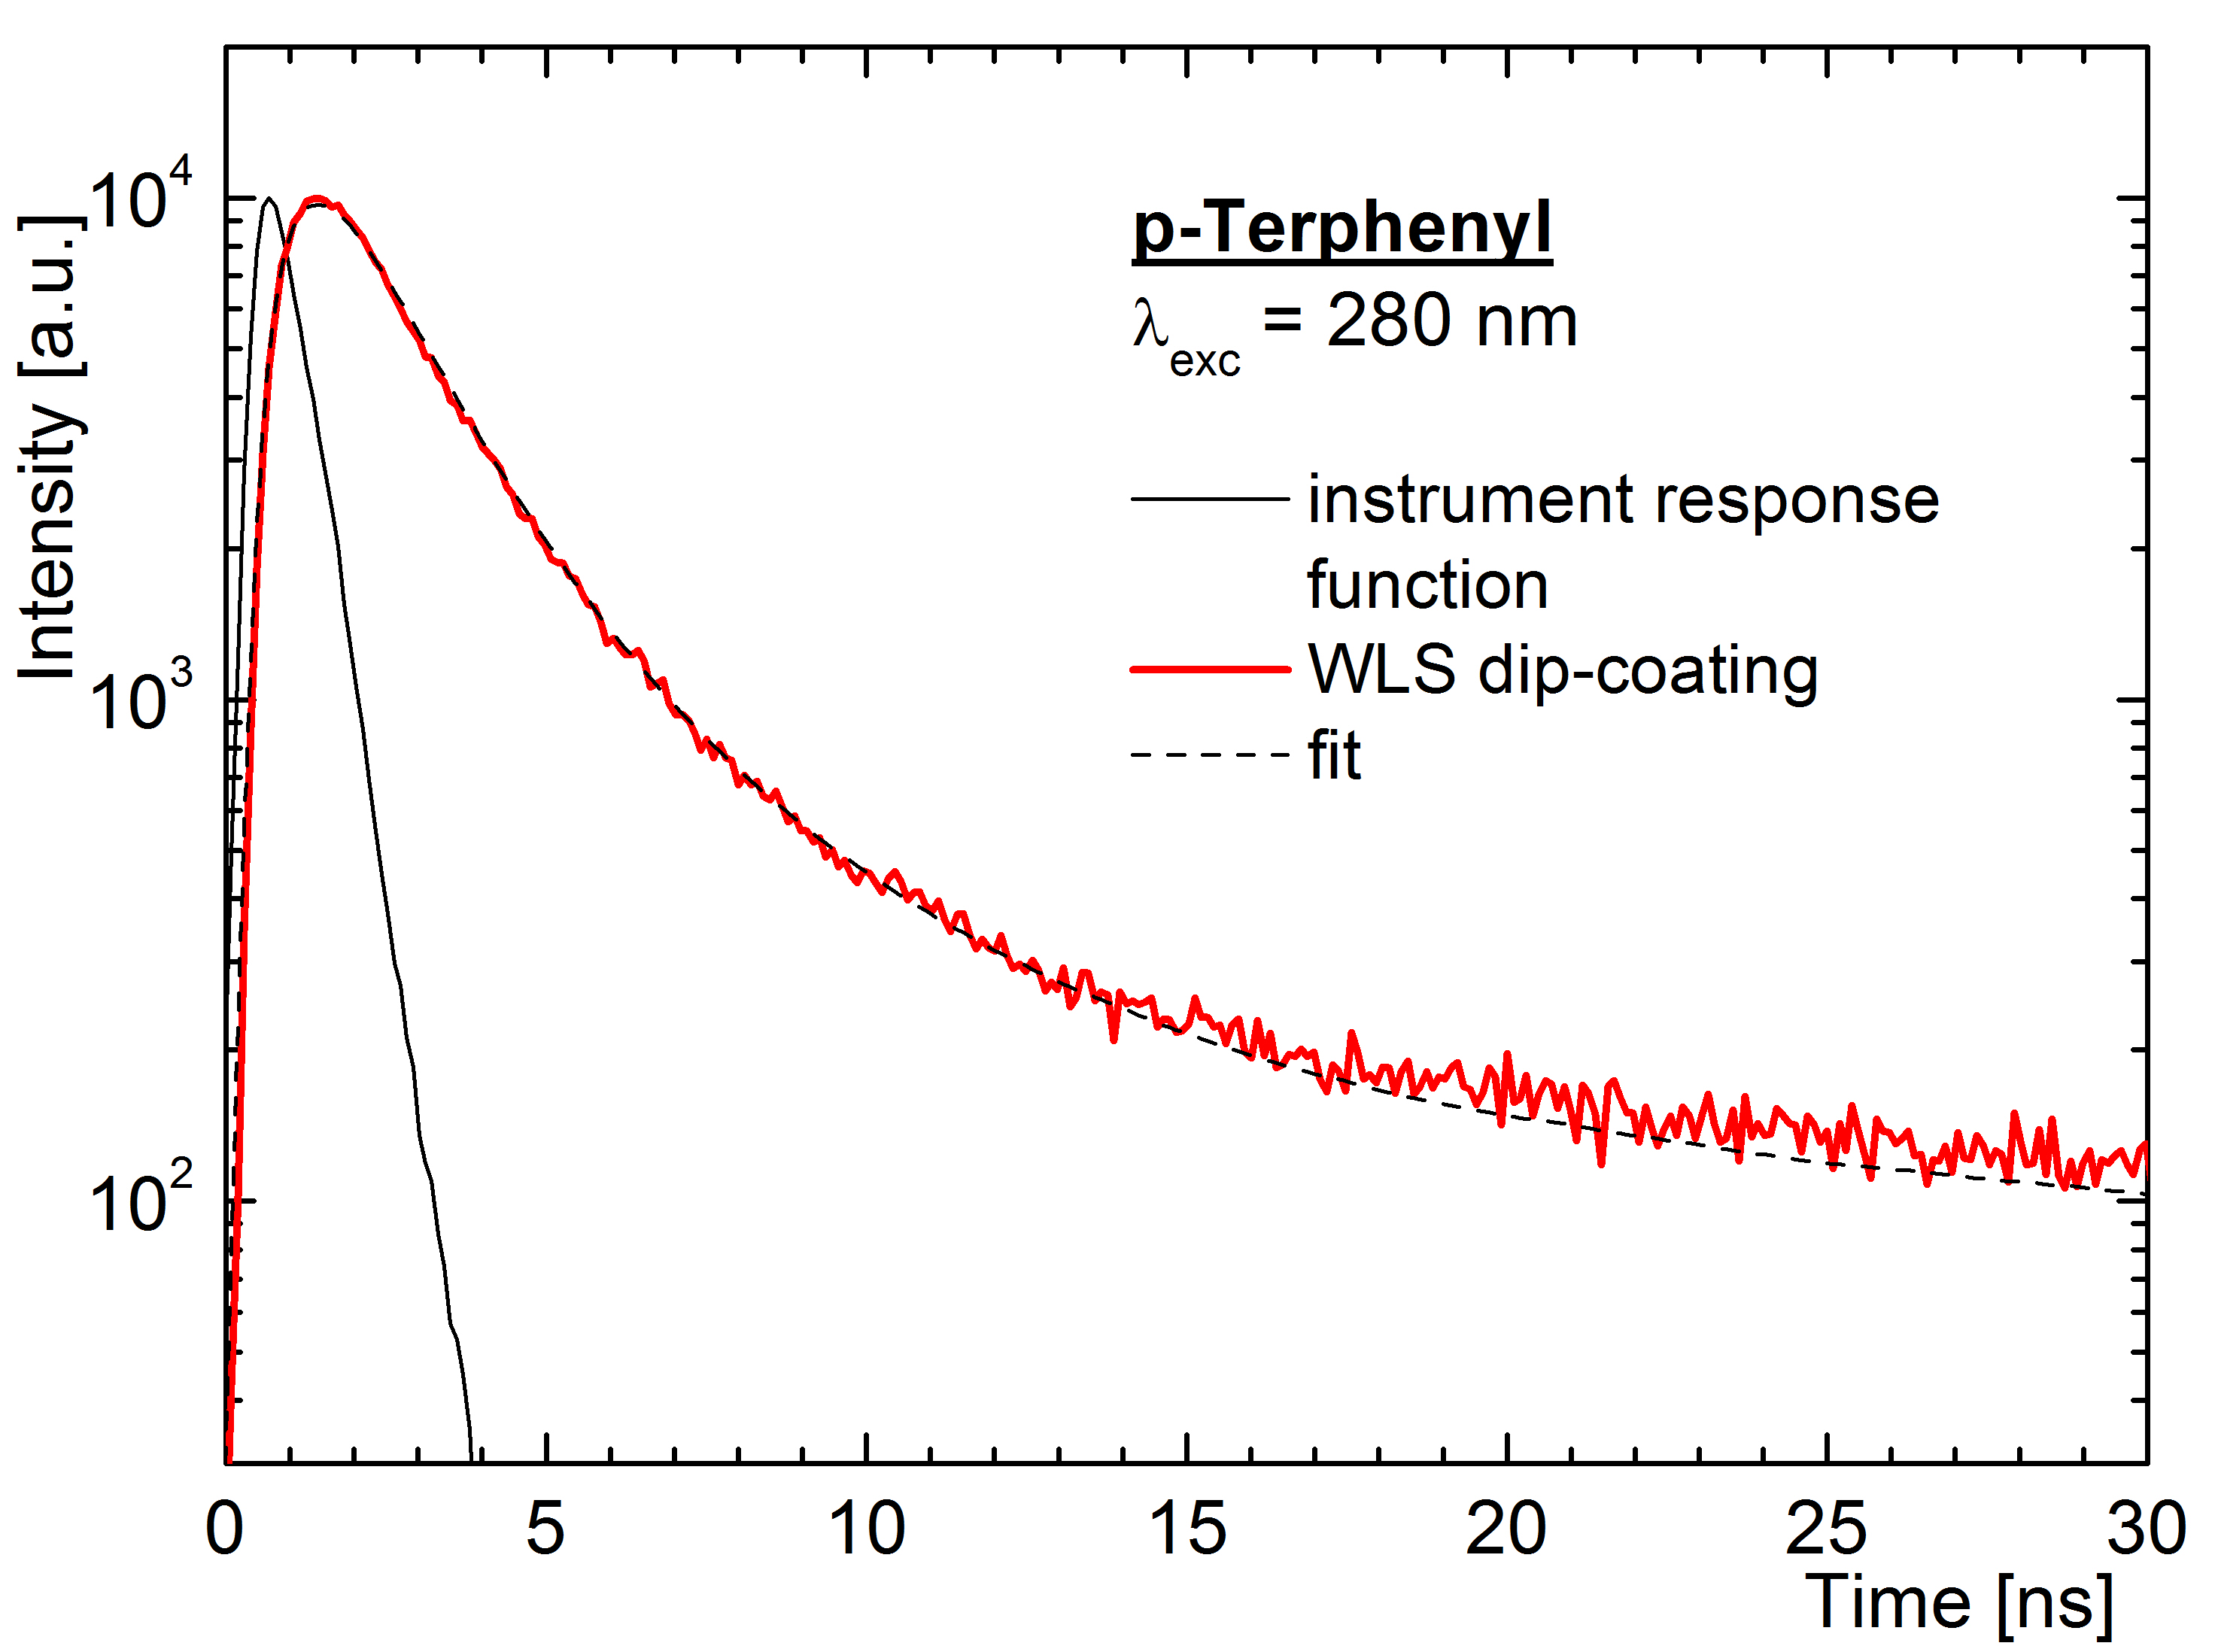
\includegraphics[width=1.0\textwidth]{pictures/Tau_fluoro_WLS_JLU.png}
\caption{}
\label{fig:MichaelProfile}
\end{figure}

Данный фит неплохо воспроизводится функцией

{\centering
$ f(t) = 10 \cdot ( A_{1} \cdot e^{-(t-1) / \tau_{1}} + A_{2} \cdot e^{-(t-1) / \tau_{2}} + A_{3} \cdot e^{-(t-1) / \tau_{3}} ) $ \\
}

со значениями амплитуд и времён, приведёнными в таблице~\ref{tabl:MichaelValues}. Здесь единица в скобке возле переменной $ t $ означает сдвиг графика по горизонтали на 1~нс и обусловлена разрешением измерительного прибора.

\begin{figure}[H]
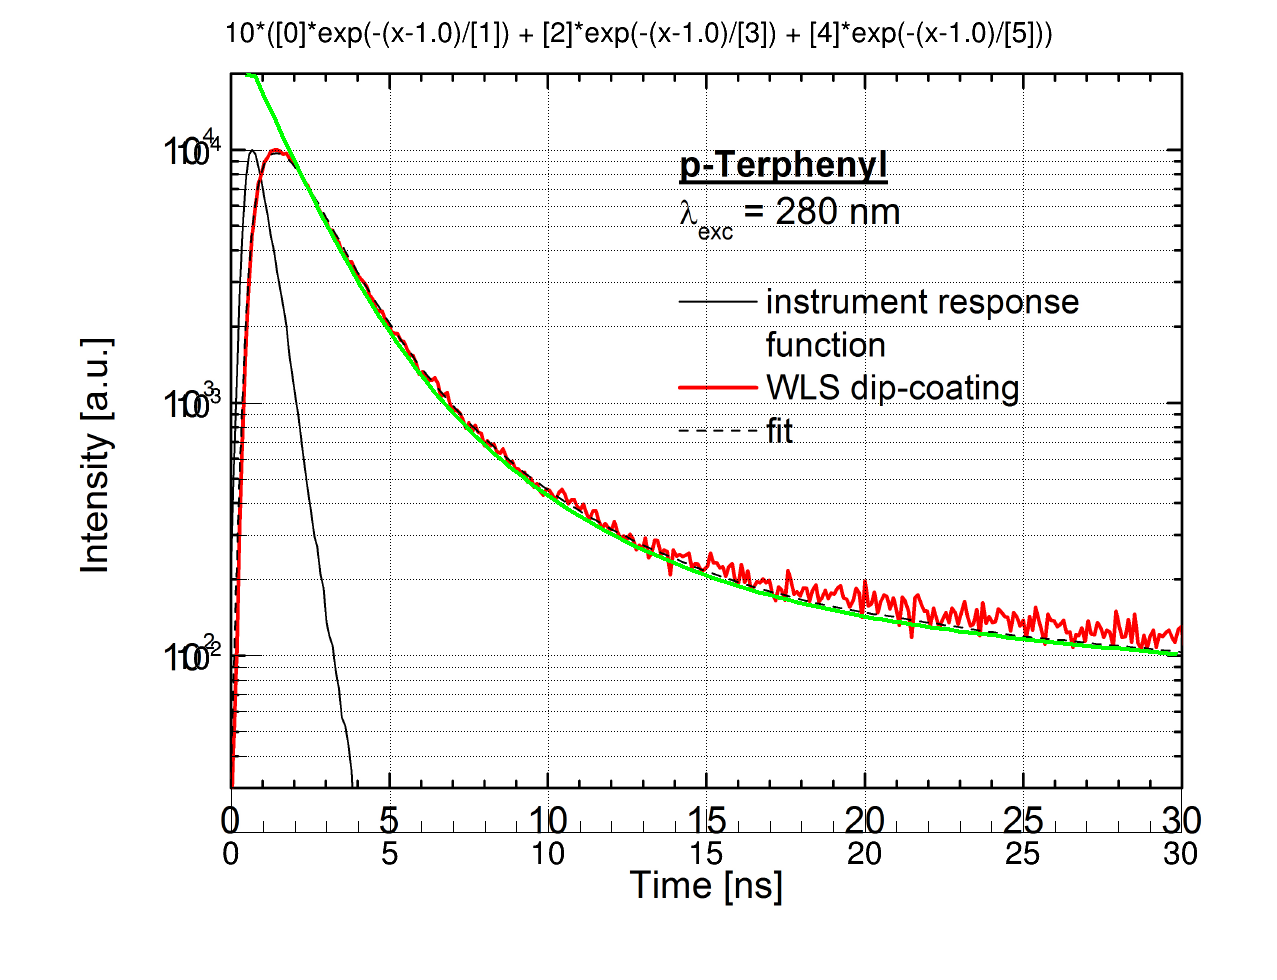
\includegraphics[width=1.0\textwidth]{pictures/FluoroFitting_shift_1ns_2.png}
\caption{}
\label{fig:MichaelProfileFit}
\end{figure}

% -----------------------------------------------------------------------------------------------

\subsection{Прямые измерения временного профиля спектросместителя}

Можно фитировать распределение WLS\textunderscore on или WLS\textunderscore off 4-мя компонентами, а можно фитировать их разницу WLS\textunderscore diff трёмя компонентами. Можно фитировать функцией с зафиксированными временами, чтобы определить амплитуды, а можно фитировать функцией, где параметрами являются и времена и амплитуды.

\subsubsection{Прямые фотоны}

В результате анализа экспериментальных данных были получены две гистограммы --- с и без сместителя спектра. Первый этап --- фитирование профиля без сместителя спектра. В результате фитирования одной экспонентой в различных диапазонах и с различными начальными условиями было получено значение временной постоянной 0.65~нс.

\begin{figure}[H]
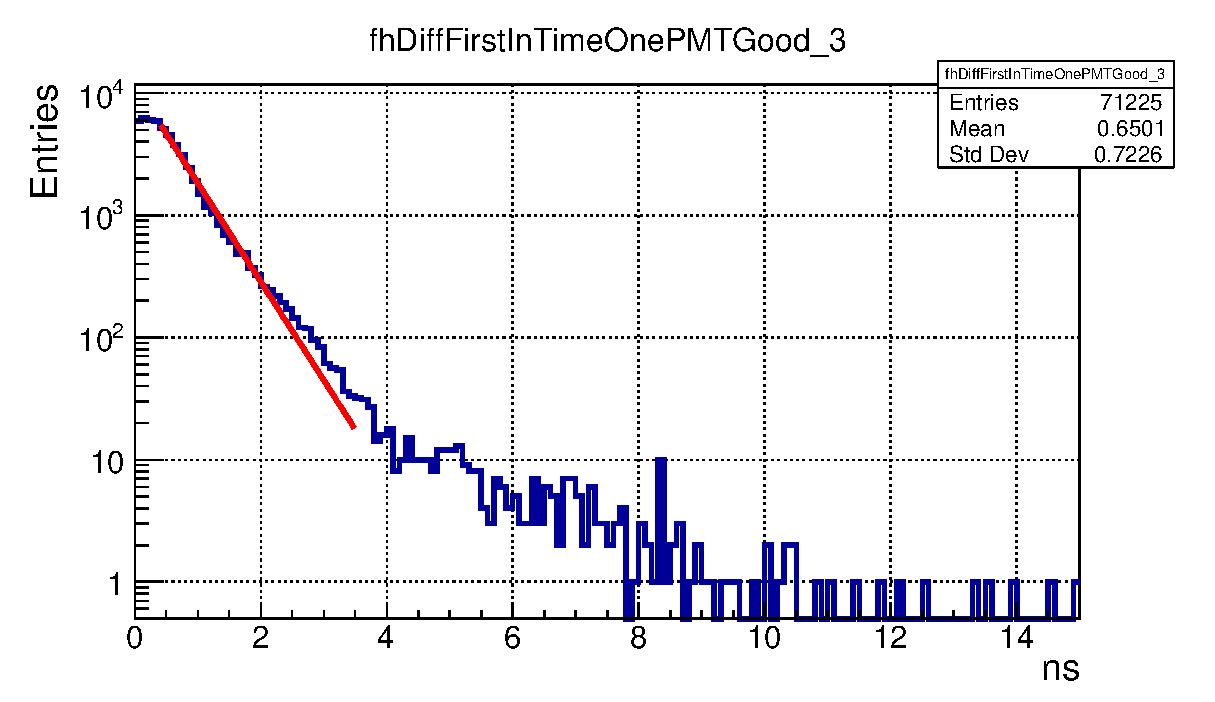
\includegraphics[width=1.0\textwidth]{pictures/WLS_off_fitting.eps}
\caption{}
\label{fig:DirectPhotons}
\end{figure}

\subsubsection{Фитирование WLS\textunderscore diff}

\begin{figure}[H]
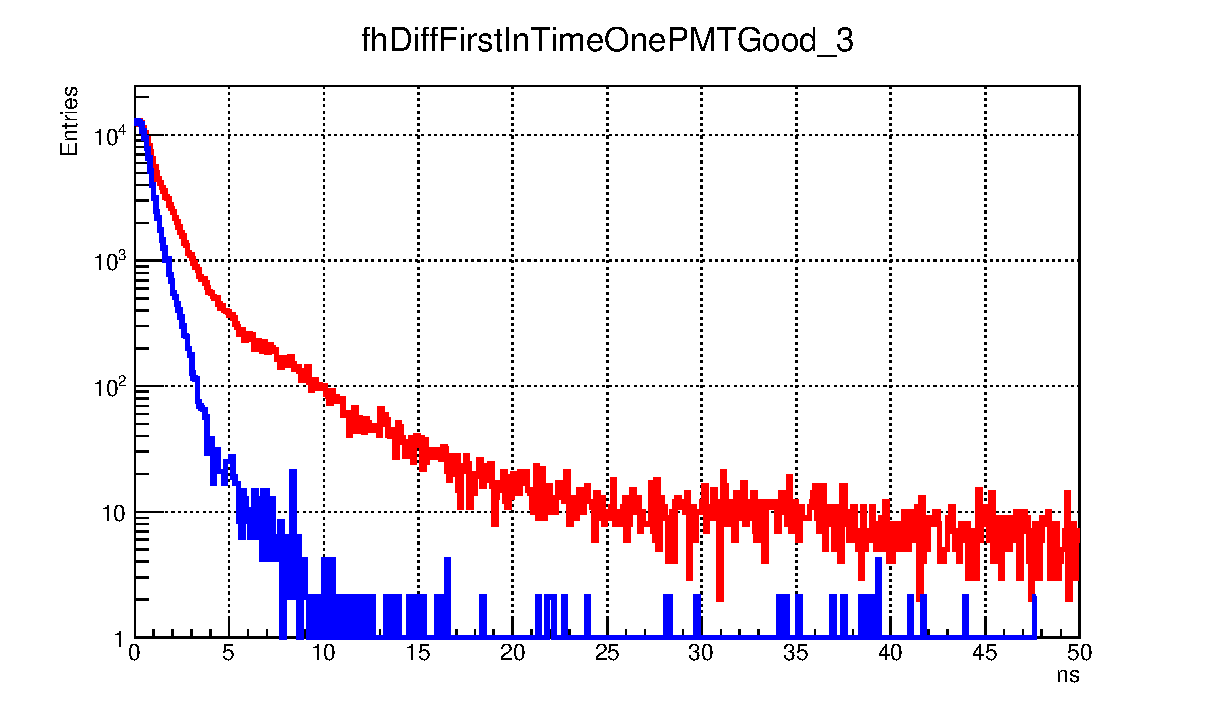
\includegraphics[width=1.0\textwidth]{pictures/WLS_curves.eps}
\caption{}
\label{fig:WlsCurves}
\end{figure}

\begin{figure}[H]
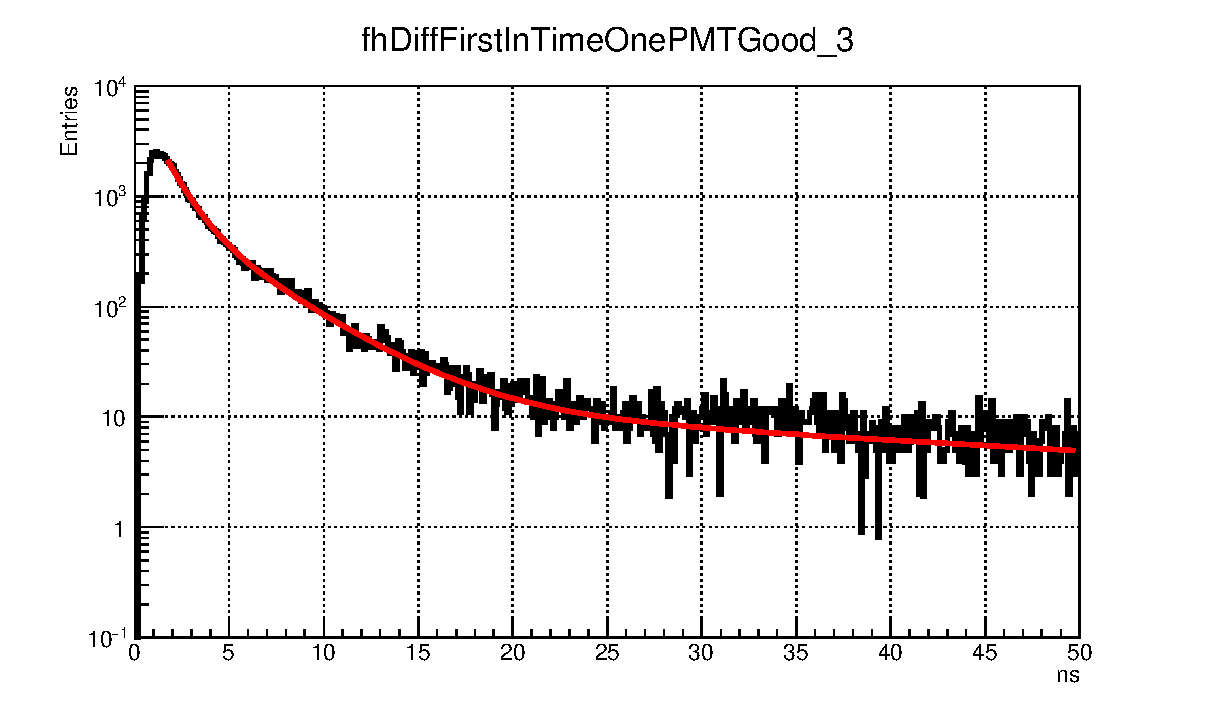
\includegraphics[width=1.0\textwidth]{pictures/diff_tripleTauFit_code682_1_1ns.eps}
\caption{}
\label{fig:WlsDiff}
\end{figure}